% Introducción

\chapter{Puesta en producción y conclusiones}

Habiendo desarrollado y validado los modelos de detección y segmentación de tumores, se procedió a poner en producción ambos modelos. Esto se llevó a cabo en etapas:

\begin{itemize}

\item construcción de API para detección
\item construcción de API para segmentación
\item construcción de front end sencillo
\item dockerización.
\end{itemize}

El flujo de información sería el siguiente:

\begin{enumerate}
    \item se carga una imagen 
    \item la imagen se guarda y se da la opción de cargar otra o procesarla con el primer modelo para detectar un tumor
    \item si el tumor es detectado, se informa y se da la opción de aplicar el modelo de segmentación, mostrando la imagen con la máscara predicha
    \item si el tumor no es detectado y se solicita su segmentación, se informa que no hay tumor a segmentar.
\end{enumerate}

A continuación se muestran imágenes del front end desarrollado y el procesamiento en la Fig. \ref{fig.web}.

El diseño del front end y back end responden al Modelo Vista Controlador usando FastAPI. Los detalles están en el Github. 

\begin{figure}[H]
    \centering
    \begin{subfigure}[b]{0.45\textwidth}
        \centering
        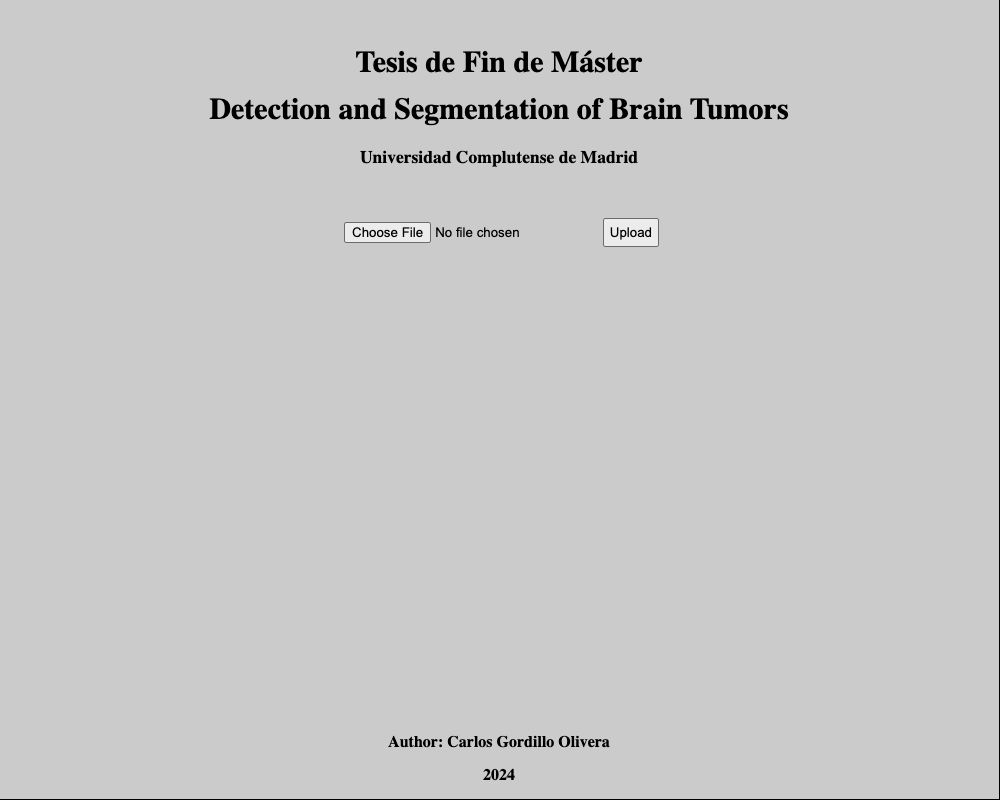
\includegraphics[width=\textwidth]{chapters/api/images/home.png}
        \caption{Vista inicial}
        \label{fig:imagen1}
    \end{subfigure}
    \hfill
    \begin{subfigure}[b]{0.45\textwidth}
        \centering
        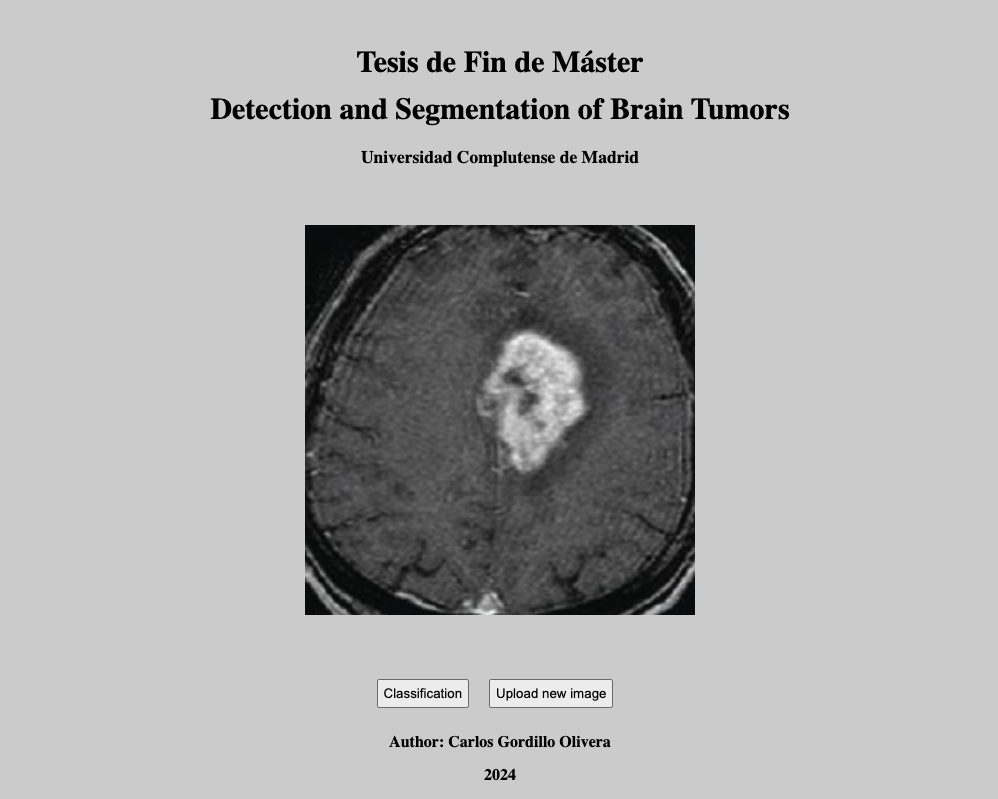
\includegraphics[width=\textwidth]{chapters/api/images/image.png}
        \caption{Imagen cargada}
        \label{fig:imagen2}
    \end{subfigure}
    
    \vspace{0.5cm} % Espacio vertical adicional entre las filas
    
    \begin{subfigure}[b]{0.45\textwidth}
        \centering
        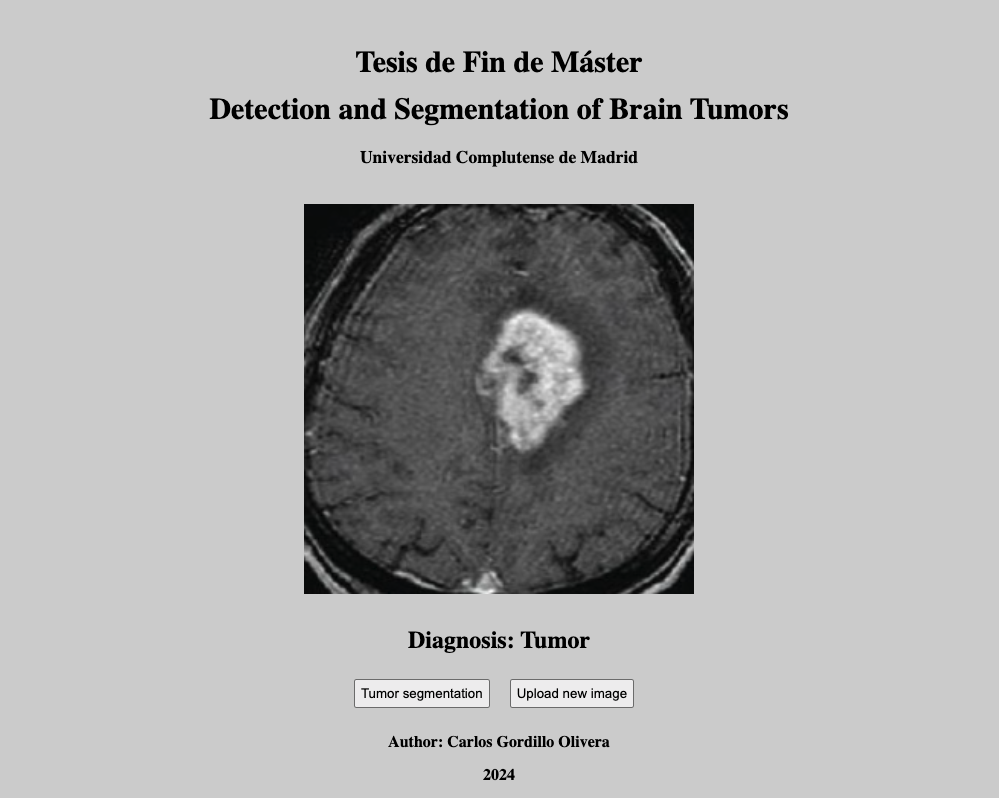
\includegraphics[width=\textwidth]{chapters/api/images/deteccion.png}
        \caption{Resultado de la detección}
        \label{fig:imagen3}
    \end{subfigure}
    \hfill
    \begin{subfigure}[b]{0.45\textwidth}
        \centering
        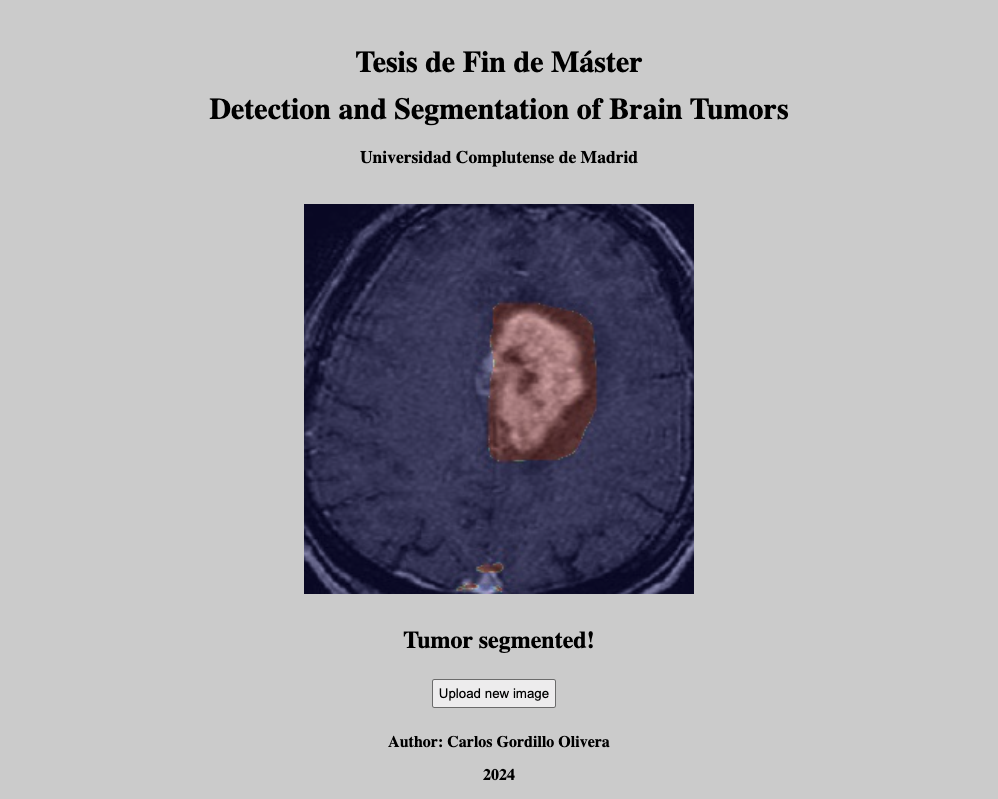
\includegraphics[width=\textwidth]{chapters/api/images/segmentacion.png}
        \caption{Resultado de la segmentación}
        \label{fig:imagen4}
    \end{subfigure}
    \caption{Flujo de información}
    \label{fig.web}
\end{figure}


Como conclusiones finales, se logró desarrollar un modelo de detección de tumores cerebrales. Dicho modelo fue evaluado y se descartó overfitting y presentó excelentes métricas de desempeño.

Se desarrolló también un modelo de segmentación de tumores, es decir, no únicamente detectar la presencia de tumores sino determinar la ubicación de los mismos. Se lo evaluó descartando overfitting y presentó buenas métricas.

Finalmente se desarrolló una API junto con un front end con el objetivo de poner en producción ambos modelos sumado a la visualización por parte del usuario. 


